\documentclass[1p]{elsarticle_modified}
%\bibliographystyle{elsarticle-num}

%\usepackage[colorlinks]{hyperref}
%\usepackage{abbrmath_seonhwa} %\Abb, \Ascr, \Acal ,\Abf, \Afrak
\usepackage{amsfonts}
\usepackage{amssymb}
\usepackage{amsmath}
\usepackage{amsthm}
\usepackage{scalefnt}
\usepackage{amsbsy}
\usepackage{kotex}
\usepackage{caption}
\usepackage{subfig}
\usepackage{color}
\usepackage{graphicx}
\usepackage{xcolor} %% white, black, red, green, blue, cyan, magenta, yellow
\usepackage{float}
\usepackage{setspace}
\usepackage{hyperref}

\usepackage{tikz}
\usetikzlibrary{arrows}

\usepackage{multirow}
\usepackage{array} % fixed length table
\usepackage{hhline}

%%%%%%%%%%%%%%%%%%%%%
\makeatletter
\renewcommand*\env@matrix[1][\arraystretch]{%
	\edef\arraystretch{#1}%
	\hskip -\arraycolsep
	\let\@ifnextchar\new@ifnextchar
	\array{*\c@MaxMatrixCols c}}
\makeatother %https://tex.stackexchange.com/questions/14071/how-can-i-increase-the-line-spacing-in-a-matrix
%%%%%%%%%%%%%%%

\usepackage[normalem]{ulem}

\newcommand{\msout}[1]{\ifmmode\text{\sout{\ensuremath{#1}}}\else\sout{#1}\fi}
%SOURCE: \msout is \stkout macro in https://tex.stackexchange.com/questions/20609/strikeout-in-math-mode

\newcommand{\cancel}[1]{
	\ifmmode
	{\color{red}\msout{#1}}
	\else
	{\color{red}\sout{#1}}
	\fi
}

\newcommand{\add}[1]{
	{\color{blue}\uwave{#1}}
}

\newcommand{\replace}[2]{
	\ifmmode
	{\color{red}\msout{#1}}{\color{blue}\uwave{#2}}
	\else
	{\color{red}\sout{#1}}{\color{blue}\uwave{#2}}
	\fi
}

\newcommand{\Sol}{\mathcal{S}} %segment
\newcommand{\D}{D} %diagram
\newcommand{\A}{\mathcal{A}} %arc


%%%%%%%%%%%%%%%%%%%%%%%%%%%%%5 test

\def\sl{\operatorname{\textup{SL}}(2,\Cbb)}
\def\psl{\operatorname{\textup{PSL}}(2,\Cbb)}
\def\quan{\mkern 1mu \triangleright \mkern 1mu}

\theoremstyle{definition}
\newtheorem{thm}{Theorem}[section]
\newtheorem{prop}[thm]{Proposition}
\newtheorem{lem}[thm]{Lemma}
\newtheorem{ques}[thm]{Question}
\newtheorem{cor}[thm]{Corollary}
\newtheorem{defn}[thm]{Definition}
\newtheorem{exam}[thm]{Example}
\newtheorem{rmk}[thm]{Remark}
\newtheorem{alg}[thm]{Algorithm}

\newcommand{\I}{\sqrt{-1}}
\begin{document}

%\begin{frontmatter}
%
%\title{Boundary parabolic representations of knots up to 8 crossings}
%
%%% Group authors per affiliation:
%\author{Yunhi Cho} 
%\address{Department of Mathematics, University of Seoul, Seoul, Korea}
%\ead{yhcho@uos.ac.kr}
%
%
%\author{Seonhwa Kim} %\fnref{s_kim}}
%\address{Center for Geometry and Physics, Institute for Basic Science, Pohang, 37673, Korea}
%\ead{ryeona17@ibs.re.kr}
%
%\author{Hyuk Kim}
%\address{Department of Mathematical Sciences, Seoul National University, Seoul 08826, Korea}
%\ead{hyukkim@snu.ac.kr}
%
%\author{Seokbeom Yoon}
%\address{Department of Mathematical Sciences, Seoul National University, Seoul, 08826,  Korea}
%\ead{sbyoon15@snu.ac.kr}
%
%\begin{abstract}
%We find all boundary parabolic representation of knots up to 8 crossings.
%
%\end{abstract}
%\begin{keyword}
%    \MSC[2010] 57M25 
%\end{keyword}
%
%\end{frontmatter}

%\linenumbers
%\tableofcontents
%
\newcommand\colored[1]{\textcolor{white}{\rule[-0.35ex]{0.8em}{1.4ex}}\kern-0.8em\color{red} #1}%
%\newcommand\colored[1]{\textcolor{white}{ #1}\kern-2.17ex	\textcolor{white}{ #1}\kern-1.81ex	\textcolor{white}{ #1}\kern-2.15ex\color{red}#1	}

{\Large $\underline{12n_{0812}~(K12n_{0812})}$}

\setlength{\tabcolsep}{10pt}
\renewcommand{\arraystretch}{1.6}
\vspace{1cm}\begin{tabular}{m{100pt}>{\centering\arraybackslash}m{274pt}}
\multirow{5}{120pt}{
	\centering
	\includegraphics[width=112pt]{../../../GIT/diagram.site/Diagrams/png/2901_12n_0812.png}\\
\ \ \ A knot diagram\footnotemark}&
\allowdisplaybreaks
\textbf{Linearized knot diagam} \\
\cline{2-2}
 &
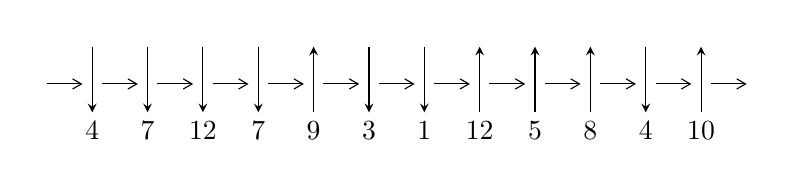
\begin{tikzpicture}[x=20pt, y=17pt]
	% nodes
	\node (C0) at (0, 0) {};
	\node (C1) at (1, 0) {};
	\node (C1U) at (1, +1) {};
	\node (C1D) at (1, -1) {4};

	\node (C2) at (2, 0) {};
	\node (C2U) at (2, +1) {};
	\node (C2D) at (2, -1) {7};

	\node (C3) at (3, 0) {};
	\node (C3U) at (3, +1) {};
	\node (C3D) at (3, -1) {12};

	\node (C4) at (4, 0) {};
	\node (C4U) at (4, +1) {};
	\node (C4D) at (4, -1) {7};

	\node (C5) at (5, 0) {};
	\node (C5U) at (5, +1) {};
	\node (C5D) at (5, -1) {9};

	\node (C6) at (6, 0) {};
	\node (C6U) at (6, +1) {};
	\node (C6D) at (6, -1) {3};

	\node (C7) at (7, 0) {};
	\node (C7U) at (7, +1) {};
	\node (C7D) at (7, -1) {1};

	\node (C8) at (8, 0) {};
	\node (C8U) at (8, +1) {};
	\node (C8D) at (8, -1) {12};

	\node (C9) at (9, 0) {};
	\node (C9U) at (9, +1) {};
	\node (C9D) at (9, -1) {5};

	\node (C10) at (10, 0) {};
	\node (C10U) at (10, +1) {};
	\node (C10D) at (10, -1) {8};

	\node (C11) at (11, 0) {};
	\node (C11U) at (11, +1) {};
	\node (C11D) at (11, -1) {4};

	\node (C12) at (12, 0) {};
	\node (C12U) at (12, +1) {};
	\node (C12D) at (12, -1) {10};
	\node (C13) at (13, 0) {};

	% arrows
	\draw[->,>={angle 60}]
	(C0) edge (C1) (C1) edge (C2) (C2) edge (C3) (C3) edge (C4) (C4) edge (C5) (C5) edge (C6) (C6) edge (C7) (C7) edge (C8) (C8) edge (C9) (C9) edge (C10) (C10) edge (C11) (C11) edge (C12) (C12) edge (C13) ;	\draw[->,>=stealth]
	(C1U) edge (C1D) (C2U) edge (C2D) (C3U) edge (C3D) (C4U) edge (C4D) (C5D) edge (C5U) (C6U) edge (C6D) (C7U) edge (C7D) (C8D) edge (C8U) (C9D) edge (C9U) (C10D) edge (C10U) (C11U) edge (C11D) (C12D) edge (C12U) ;
	\end{tikzpicture} \\
\hhline{~~} \\& 
\textbf{Solving Sequence} \\ \cline{2-2} 
 &
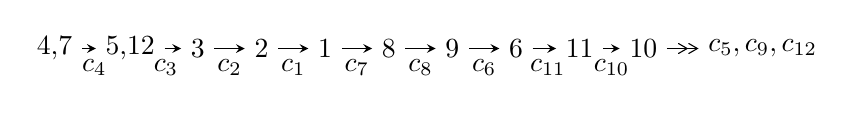
\begin{tikzpicture}[x=23pt, y=7pt]
	% node
	\node (A0) at (-1/8, 0) {4,7};
	\node (A1) at (17/16, 0) {5,12};
	\node (A2) at (17/8, 0) {3};
	\node (A3) at (25/8, 0) {2};
	\node (A4) at (33/8, 0) {1};
	\node (A5) at (41/8, 0) {8};
	\node (A6) at (49/8, 0) {9};
	\node (A7) at (57/8, 0) {6};
	\node (A8) at (65/8, 0) {11};
	\node (A9) at (73/8, 0) {10};
	\node (C1) at (1/2, -1) {$c_{4}$};
	\node (C2) at (13/8, -1) {$c_{3}$};
	\node (C3) at (21/8, -1) {$c_{2}$};
	\node (C4) at (29/8, -1) {$c_{1}$};
	\node (C5) at (37/8, -1) {$c_{7}$};
	\node (C6) at (45/8, -1) {$c_{8}$};
	\node (C7) at (53/8, -1) {$c_{6}$};
	\node (C8) at (61/8, -1) {$c_{11}$};
	\node (C9) at (69/8, -1) {$c_{10}$};
	\node (A10) at (11, 0) {$c_{5},c_{9},c_{12}$};

	% edge
	\draw[->,>=stealth]	
	(A0) edge (A1) (A1) edge (A2) (A2) edge (A3) (A3) edge (A4) (A4) edge (A5) (A5) edge (A6) (A6) edge (A7) (A7) edge (A8) (A8) edge (A9) ;
	\draw[->>,>={angle 60}]	
	(A9) edge (A10);
\end{tikzpicture} \\ 

\end{tabular} \\

\footnotetext{
The image of knot diagram is generated by the software ``\textbf{Draw programme}" developed by Andrew Bartholomew(\url{http://www.layer8.co.uk/maths/draw/index.htm\#Running-draw}), where we modified some parts for our purpose(\url{https://github.com/CATsTAILs/LinksPainter}).
}\phantom \\ \newline 
\centering \textbf{Ideals for irreducible components\footnotemark of $X_{\text{par}}$} 
 
\begin{align*}
I^u_{1}&=\langle 
-8.62027\times10^{76} u^{27}+1.52401\times10^{78} u^{26}+\cdots+1.53506\times10^{82} b+5.13581\times10^{81},\\
\phantom{I^u_{1}}&\phantom{= \langle  }1.24052\times10^{82} u^{27}+6.32881\times10^{82} u^{26}+\cdots+1.32476\times10^{85} a-4.03731\times10^{85},\\
\phantom{I^u_{1}}&\phantom{= \langle  }u^{28}+5 u^{27}+\cdots-4802 u+863\rangle \\
I^u_{2}&=\langle 
1.13096\times10^{16} u^{20}-6.66784\times10^{16} u^{19}+\cdots+3.05068\times10^{16} b-2.79012\times10^{16},\\
\phantom{I^u_{2}}&\phantom{= \langle  }8.06048\times10^{16} u^{20}-5.63230\times10^{17} u^{19}+\cdots+3.05068\times10^{16} a+3.72544\times10^{17},\;u^{21}-7 u^{20}+\cdots+7 u-1\rangle \\
I^u_{3}&=\langle 
b- u+1,\;a+u,\;u^2+1\rangle \\
I^u_{4}&=\langle 
b,\;a-1,\;u-1\rangle \\
\\
\end{align*}
\raggedright * 4 irreducible components of $\dim_{\mathbb{C}}=0$, with total 52 representations.\\
\footnotetext{All coefficients of polynomials are rational numbers. But the coefficients are sometimes approximated in decimal forms when there is not enough margin.}
\newpage
\renewcommand{\arraystretch}{1}
\centering \section*{I. $I^u_{1}= \langle -8.62\times10^{76} u^{27}+1.52\times10^{78} u^{26}+\cdots+1.54\times10^{82} b+5.14\times10^{81},\;1.24\times10^{82} u^{27}+6.33\times10^{82} u^{26}+\cdots+1.32\times10^{85} a-4.04\times10^{85},\;u^{28}+5 u^{27}+\cdots-4802 u+863 \rangle$}
\flushleft \textbf{(i) Arc colorings}\\
\begin{tabular}{m{7pt} m{180pt} m{7pt} m{180pt} }
\flushright $a_{4}=$&$\begin{pmatrix}1\\0\end{pmatrix}$ \\
\flushright $a_{7}=$&$\begin{pmatrix}0\\u\end{pmatrix}$ \\
\flushright $a_{5}=$&$\begin{pmatrix}1\\u^2\end{pmatrix}$ \\
\flushright $a_{12}=$&$\begin{pmatrix}-0.000936413 u^{27}-0.00477733 u^{26}+\cdots-8.38766 u+3.04758\\5.61558\times10^{-6} u^{27}-0.0000992801 u^{26}+\cdots-1.45523 u-0.334567\end{pmatrix}$ \\
\flushright $a_{3}=$&$\begin{pmatrix}-0.000263039 u^{27}-0.00140121 u^{26}+\cdots-1.03847 u+2.73441\\-0.000341879 u^{27}-0.00168333 u^{26}+\cdots-3.68231 u+0.495730\end{pmatrix}$ \\
\flushright $a_{2}=$&$\begin{pmatrix}-0.000263039 u^{27}-0.00140121 u^{26}+\cdots-1.03847 u+2.73441\\-0.000260254 u^{27}-0.00132797 u^{26}+\cdots-3.49625 u+0.421496\end{pmatrix}$ \\
\flushright $a_{1}=$&$\begin{pmatrix}-0.000523293 u^{27}-0.00272919 u^{26}+\cdots-4.53472 u+3.15591\\-0.000260254 u^{27}-0.00132797 u^{26}+\cdots-3.49625 u+0.421496\end{pmatrix}$ \\
\flushright $a_{8}=$&$\begin{pmatrix}0.000610060 u^{27}+0.00328680 u^{26}+\cdots+2.78600 u-1.92051\\0.000182108 u^{27}+0.00106951 u^{26}+\cdots+2.73273 u-0.211107\end{pmatrix}$ \\
\flushright $a_{9}=$&$\begin{pmatrix}0.000559019 u^{27}+0.00284931 u^{26}+\cdots+3.47453 u-1.66495\\-0.000130430 u^{27}-0.000448498 u^{26}+\cdots+1.08342 u-0.0158707\end{pmatrix}$ \\
\flushright $a_{6}=$&$\begin{pmatrix}-0.000175320 u^{27}-0.000769585 u^{26}+\cdots+1.01760 u+1.26490\\-0.0000404126 u^{27}-0.000267309 u^{26}+\cdots-0.405692 u+0.352147\end{pmatrix}$ \\
\flushright $a_{11}=$&$\begin{pmatrix}-0.000930798 u^{27}-0.00487661 u^{26}+\cdots-9.84289 u+2.71301\\5.61558\times10^{-6} u^{27}-0.0000992801 u^{26}+\cdots-1.45523 u-0.334567\end{pmatrix}$ \\
\flushright $a_{10}=$&$\begin{pmatrix}-0.000726886 u^{27}-0.00405664 u^{26}+\cdots-4.78005 u+1.63403\\-0.0000519443 u^{27}-0.000325470 u^{26}+\cdots-2.70568 u+0.333453\end{pmatrix}$\\&\end{tabular}
\flushleft \textbf{(ii) Obstruction class $= -1$}\\~\\
\flushleft \textbf{(iii) Cusp Shapes $= 0.00191539 u^{27}+0.00980758 u^{26}+\cdots+12.3575 u-10.5692$}\\~\\
\newpage\renewcommand{\arraystretch}{1}
\flushleft \textbf{(iv) u-Polynomials at the component}\newline \\
\begin{tabular}{m{50pt}|m{274pt}}
Crossings & \hspace{64pt}u-Polynomials at each crossing \\
\hline $$\begin{aligned}c_{1}\end{aligned}$$&$\begin{aligned}
&u^{28}-4 u^{27}+\cdots+167 u-43
\end{aligned}$\\
\hline $$\begin{aligned}c_{2},c_{6}\end{aligned}$$&$\begin{aligned}
&u^{28}+2 u^{27}+\cdots+207872 u-13157
\end{aligned}$\\
\hline $$\begin{aligned}c_{3},c_{11}\end{aligned}$$&$\begin{aligned}
&u^{28}-9 u^{27}+\cdots+10968 u-4784
\end{aligned}$\\
\hline $$\begin{aligned}c_{4}\end{aligned}$$&$\begin{aligned}
&u^{28}-5 u^{27}+\cdots+4802 u+863
\end{aligned}$\\
\hline $$\begin{aligned}c_{5},c_{9}\end{aligned}$$&$\begin{aligned}
&u^{28}+13 u^{26}+\cdots-2972 u-4630
\end{aligned}$\\
\hline $$\begin{aligned}c_{7}\end{aligned}$$&$\begin{aligned}
&u^{28}-3 u^{27}+\cdots+56 u-8
\end{aligned}$\\
\hline $$\begin{aligned}c_{8}\end{aligned}$$&$\begin{aligned}
&u^{28}+u^{27}+\cdots+9495203 u+439429
\end{aligned}$\\
\hline $$\begin{aligned}c_{10}\end{aligned}$$&$\begin{aligned}
&u^{28}- u^{27}+\cdots+14900 u-3331
\end{aligned}$\\
\hline $$\begin{aligned}c_{12}\end{aligned}$$&$\begin{aligned}
&u^{28}+4 u^{27}+\cdots-100 u-25
\end{aligned}$\\
\hline
\end{tabular}\\~\\
\newpage\renewcommand{\arraystretch}{1}
\flushleft \textbf{(v) Riley Polynomials at the component}\newline \\
\begin{tabular}{m{50pt}|m{274pt}}
Crossings & \hspace{64pt}Riley Polynomials at each crossing \\
\hline $$\begin{aligned}c_{1}\end{aligned}$$&$\begin{aligned}
&y^{28}-58 y^{27}+\cdots-24449 y+1849
\end{aligned}$\\
\hline $$\begin{aligned}c_{2},c_{6}\end{aligned}$$&$\begin{aligned}
&y^{28}+60 y^{27}+\cdots-31398071702 y+173106649
\end{aligned}$\\
\hline $$\begin{aligned}c_{3},c_{11}\end{aligned}$$&$\begin{aligned}
&y^{28}+37 y^{27}+\cdots-349087040 y+22886656
\end{aligned}$\\
\hline $$\begin{aligned}c_{4}\end{aligned}$$&$\begin{aligned}
&y^{28}-21 y^{27}+\cdots-7045376 y+744769
\end{aligned}$\\
\hline $$\begin{aligned}c_{5},c_{9}\end{aligned}$$&$\begin{aligned}
&y^{28}+26 y^{27}+\cdots+2260696 y+21436900
\end{aligned}$\\
\hline $$\begin{aligned}c_{7}\end{aligned}$$&$\begin{aligned}
&y^{28}+11 y^{27}+\cdots-768 y+64
\end{aligned}$\\
\hline $$\begin{aligned}c_{8}\end{aligned}$$&$\begin{aligned}
&y^{28}-85 y^{27}+\cdots-41732534261399 y+193097846041
\end{aligned}$\\
\hline $$\begin{aligned}c_{10}\end{aligned}$$&$\begin{aligned}
&y^{28}-51 y^{27}+\cdots-22556382 y+11095561
\end{aligned}$\\
\hline $$\begin{aligned}c_{12}\end{aligned}$$&$\begin{aligned}
&y^{28}-6 y^{27}+\cdots-10150 y+625
\end{aligned}$\\
\hline
\end{tabular}\\~\\
\newpage\flushleft \textbf{(vi) Complex Volumes and Cusp Shapes}
$$\begin{array}{c|c|c}  
\text{Solutions to }I^u_{1}& \I (\text{vol} + \sqrt{-1}CS) & \text{Cusp shape}\\
 \hline 
\begin{aligned}
u &= -0.459433 + 1.004210 I \\
a &= -0.769069 - 0.424094 I \\
b &= \phantom{-}2.01354 + 1.09433 I\end{aligned}
 & -10.03210 - 2.03721 I & \phantom{-}1.40807 + 1.51569 I \\ \hline\begin{aligned}
u &= -0.459433 - 1.004210 I \\
a &= -0.769069 + 0.424094 I \\
b &= \phantom{-}2.01354 - 1.09433 I\end{aligned}
 & -10.03210 + 2.03721 I & \phantom{-}1.40807 - 1.51569 I \\ \hline\begin{aligned}
u &= \phantom{-}0.273744 + 0.828909 I \\
a &= -0.31857 - 1.39833 I \\
b &= \phantom{-}0.676810 + 0.678060 I\end{aligned}
 & \phantom{-}3.25948 + 1.87994 I & \phantom{-}1.127245 + 0.255189 I \\ \hline\begin{aligned}
u &= \phantom{-}0.273744 - 0.828909 I \\
a &= -0.31857 + 1.39833 I \\
b &= \phantom{-}0.676810 - 0.678060 I\end{aligned}
 & \phantom{-}3.25948 - 1.87994 I & \phantom{-}1.127245 - 0.255189 I \\ \hline\begin{aligned}
u &= \phantom{-}0.229511 + 0.822937 I \\
a &= \phantom{-}0.524171 + 0.383309 I \\
b &= \phantom{-}0.390248 - 0.173189 I\end{aligned}
 & \phantom{-}0.13617 - 2.17117 I & -0.52994 + 4.56699 I \\ \hline\begin{aligned}
u &= \phantom{-}0.229511 - 0.822937 I \\
a &= \phantom{-}0.524171 - 0.383309 I \\
b &= \phantom{-}0.390248 + 0.173189 I\end{aligned}
 & \phantom{-}0.13617 + 2.17117 I & -0.52994 - 4.56699 I \\ \hline\begin{aligned}
u &= \phantom{-}0.822714\phantom{ +0.000000I} \\
a &= \phantom{-}0.146759\phantom{ +0.000000I} \\
b &= -0.732140\phantom{ +0.000000I}\end{aligned}
 & -1.55304\phantom{ +0.000000I} & -5.27900\phantom{ +0.000000I} \\ \hline\begin{aligned}
u &= \phantom{-}0.836672 + 0.864882 I \\
a &= -0.56617 + 1.86096 I \\
b &= -0.562756 - 0.399087 I\end{aligned}
 & \phantom{-}1.97057 - 6.52494 I & -1.83111 + 8.72203 I \\ \hline\begin{aligned}
u &= \phantom{-}0.836672 - 0.864882 I \\
a &= -0.56617 - 1.86096 I \\
b &= -0.562756 + 0.399087 I\end{aligned}
 & \phantom{-}1.97057 + 6.52494 I & -1.83111 - 8.72203 I \\ \hline\begin{aligned}
u &= -0.480459 + 0.282436 I \\
a &= \phantom{-}1.41640 + 0.49816 I \\
b &= \phantom{-}0.516137 - 0.268437 I\end{aligned}
 & \phantom{-}1.51898 - 0.09189 I & \phantom{-}7.42707 - 0.14730 I\\
 \hline 
 \end{array}$$\newpage$$\begin{array}{c|c|c}  
\text{Solutions to }I^u_{1}& \I (\text{vol} + \sqrt{-1}CS) & \text{Cusp shape}\\
 \hline 
\begin{aligned}
u &= -0.480459 - 0.282436 I \\
a &= \phantom{-}1.41640 - 0.49816 I \\
b &= \phantom{-}0.516137 + 0.268437 I\end{aligned}
 & \phantom{-}1.51898 + 0.09189 I & \phantom{-}7.42707 + 0.14730 I \\ \hline\begin{aligned}
u &= -0.43263 + 1.42005 I \\
a &= -0.322046 - 1.165460 I \\
b &= -0.08622 + 2.09948 I\end{aligned}
 & \phantom{-}11.60450 + 1.52928 I & \phantom{-}5.96173 - 5.20161 I \\ \hline\begin{aligned}
u &= -0.43263 - 1.42005 I \\
a &= -0.322046 + 1.165460 I \\
b &= -0.08622 - 2.09948 I\end{aligned}
 & \phantom{-}11.60450 - 1.52928 I & \phantom{-}5.96173 + 5.20161 I \\ \hline\begin{aligned}
u &= \phantom{-}1.36989 + 0.62388 I \\
a &= -0.522052 - 0.287024 I \\
b &= -0.856845 + 0.272486 I\end{aligned}
 & -2.93559 - 3.60574 I & -2.03784 + 5.31911 I \\ \hline\begin{aligned}
u &= \phantom{-}1.36989 - 0.62388 I \\
a &= -0.522052 + 0.287024 I \\
b &= -0.856845 - 0.272486 I\end{aligned}
 & -2.93559 + 3.60574 I & -2.03784 - 5.31911 I \\ \hline\begin{aligned}
u &= \phantom{-}0.216176 + 0.152550 I \\
a &= \phantom{-}1.23983 - 1.38812 I \\
b &= -0.694421 - 0.417839 I\end{aligned}
 & -1.34198 - 0.63181 I & -7.39383 + 3.55585 I \\ \hline\begin{aligned}
u &= \phantom{-}0.216176 - 0.152550 I \\
a &= \phantom{-}1.23983 + 1.38812 I \\
b &= -0.694421 + 0.417839 I\end{aligned}
 & -1.34198 + 0.63181 I & -7.39383 - 3.55585 I \\ \hline\begin{aligned}
u &= \phantom{-}1.55762 + 0.81392 I \\
a &= \phantom{-}0.785031 - 0.314648 I \\
b &= \phantom{-}0.41609 + 1.75558 I\end{aligned}
 & \phantom{-}2.40615 - 3.22239 I & \phantom{-}0.05887 + 2.24675 I \\ \hline\begin{aligned}
u &= \phantom{-}1.55762 - 0.81392 I \\
a &= \phantom{-}0.785031 + 0.314648 I \\
b &= \phantom{-}0.41609 - 1.75558 I\end{aligned}
 & \phantom{-}2.40615 + 3.22239 I & \phantom{-}0.05887 - 2.24675 I \\ \hline\begin{aligned}
u &= -1.73297 + 0.36682 I \\
a &= \phantom{-}0.207455 - 0.021422 I \\
b &= -0.093173 - 1.202150 I\end{aligned}
 & -3.72120 + 5.07083 I & -0.01986 - 3.99214 I\\
 \hline 
 \end{array}$$\newpage$$\begin{array}{c|c|c}  
\text{Solutions to }I^u_{1}& \I (\text{vol} + \sqrt{-1}CS) & \text{Cusp shape}\\
 \hline 
\begin{aligned}
u &= -1.73297 - 0.36682 I \\
a &= \phantom{-}0.207455 + 0.021422 I \\
b &= -0.093173 + 1.202150 I\end{aligned}
 & -3.72120 - 5.07083 I & -0.01986 + 3.99214 I \\ \hline\begin{aligned}
u &= -1.05080 + 2.14321 I \\
a &= \phantom{-}0.291815 + 0.781957 I \\
b &= \phantom{-}1.45524 - 3.34171 I\end{aligned}
 & \phantom{-}14.9730 + 2.7474 I & \phantom{-0.000000 } 0 \\ \hline\begin{aligned}
u &= -1.05080 - 2.14321 I \\
a &= \phantom{-}0.291815 - 0.781957 I \\
b &= \phantom{-}1.45524 + 3.34171 I\end{aligned}
 & \phantom{-}14.9730 - 2.7474 I & \phantom{-0.000000 } 0 \\ \hline\begin{aligned}
u &= -1.85519 + 1.64553 I \\
a &= -0.554886 - 0.593820 I \\
b &= -1.69865 + 2.55029 I\end{aligned}
 & \phantom{-}15.8138 + 12.8690 I & \phantom{-0.000000 } 0 \\ \hline\begin{aligned}
u &= -1.85519 - 1.64553 I \\
a &= -0.554886 + 0.593820 I \\
b &= -1.69865 - 2.55029 I\end{aligned}
 & \phantom{-}15.8138 - 12.8690 I & \phantom{-0.000000 } 0 \\ \hline\begin{aligned}
u &= \phantom{-}2.92172\phantom{ +0.000000I} \\
a &= \phantom{-}0.782361\phantom{ +0.000000I} \\
b &= \phantom{-}2.34197\phantom{ +0.000000I}\end{aligned}
 & -6.12420\phantom{ +0.000000I} & \phantom{-0.000000 } 0 \\ \hline\begin{aligned}
u &= -2.84436 + 1.35079 I \\
a &= \phantom{-}0.540100 + 0.227911 I \\
b &= \phantom{-}2.21908 - 3.05252 I\end{aligned}
 & \phantom{-}14.6001 + 2.0794 I & \phantom{-0.000000 } 0 \\ \hline\begin{aligned}
u &= -2.84436 - 1.35079 I \\
a &= \phantom{-}0.540100 - 0.227911 I \\
b &= \phantom{-}2.21908 + 3.05252 I\end{aligned}
 & \phantom{-}14.6001 - 2.0794 I & \phantom{-0.000000 } 0\\
 \hline 
 \end{array}$$\newpage\newpage\renewcommand{\arraystretch}{1}
\centering \section*{II. $I^u_{2}= \langle 1.13\times10^{16} u^{20}-6.67\times10^{16} u^{19}+\cdots+3.05\times10^{16} b-2.79\times10^{16},\;8.06\times10^{16} u^{20}-5.63\times10^{17} u^{19}+\cdots+3.05\times10^{16} a+3.73\times10^{17},\;u^{21}-7 u^{20}+\cdots+7 u-1 \rangle$}
\flushleft \textbf{(i) Arc colorings}\\
\begin{tabular}{m{7pt} m{180pt} m{7pt} m{180pt} }
\flushright $a_{4}=$&$\begin{pmatrix}1\\0\end{pmatrix}$ \\
\flushright $a_{7}=$&$\begin{pmatrix}0\\u\end{pmatrix}$ \\
\flushright $a_{5}=$&$\begin{pmatrix}1\\u^2\end{pmatrix}$ \\
\flushright $a_{12}=$&$\begin{pmatrix}-2.64219 u^{20}+18.4624 u^{19}+\cdots+82.2885 u-12.2118\\-0.370723 u^{20}+2.18569 u^{19}+\cdots-3.27253 u+0.914589\end{pmatrix}$ \\
\flushright $a_{3}=$&$\begin{pmatrix}2.45654 u^{20}-16.5538 u^{19}+\cdots-46.8691 u+2.84798\\-0.218854 u^{20}+1.77628 u^{19}+\cdots+6.32405 u-0.684934\end{pmatrix}$ \\
\flushright $a_{2}=$&$\begin{pmatrix}2.45654 u^{20}-16.5538 u^{19}+\cdots-46.8691 u+2.84798\\-0.399174 u^{20}+2.83676 u^{19}+\cdots+8.36141 u-1.32692\end{pmatrix}$ \\
\flushright $a_{1}=$&$\begin{pmatrix}2.05736 u^{20}-13.7170 u^{19}+\cdots-38.5077 u+1.52106\\-0.399174 u^{20}+2.83676 u^{19}+\cdots+8.36141 u-1.32692\end{pmatrix}$ \\
\flushright $a_{8}=$&$\begin{pmatrix}0.847229 u^{20}-5.50818 u^{19}+\cdots-36.8397 u+10.1554\\0.852360 u^{20}-4.81815 u^{19}+\cdots-3.93557 u-0.0851849\end{pmatrix}$ \\
\flushright $a_{9}=$&$\begin{pmatrix}-2.83718 u^{20}+20.1617 u^{19}+\cdots+69.2365 u-4.68421\\1.24144 u^{20}-7.58901 u^{19}+\cdots-14.9295 u+2.08597\end{pmatrix}$ \\
\flushright $a_{6}=$&$\begin{pmatrix}0.608465 u^{20}-3.20801 u^{19}+\cdots+25.3385 u-10.0693\\-0.0544761 u^{20}+0.450258 u^{19}+\cdots+0.815373 u+0.880016\end{pmatrix}$ \\
\flushright $a_{11}=$&$\begin{pmatrix}-3.01292 u^{20}+20.6481 u^{19}+\cdots+79.0160 u-11.2973\\-0.370723 u^{20}+2.18569 u^{19}+\cdots-3.27253 u+0.914589\end{pmatrix}$ \\
\flushright $a_{10}=$&$\begin{pmatrix}-2.82469 u^{20}+19.6190 u^{19}+\cdots+59.2542 u-2.89968\\0.763744 u^{20}-4.65415 u^{19}+\cdots-11.7302 u+1.63071\end{pmatrix}$\\&\end{tabular}
\flushleft \textbf{(ii) Obstruction class $= 1$}\\~\\
\flushleft \textbf{(iii) Cusp Shapes $= -\frac{142462361688498817}{30506810548263331} u^{20}+\frac{853512483449208650}{30506810548263331} u^{19}+\cdots+\frac{205869171519914537}{30506810548263331} u+\frac{184825108905214746}{30506810548263331}$}\\~\\
\newpage\renewcommand{\arraystretch}{1}
\flushleft \textbf{(iv) u-Polynomials at the component}\newline \\
\begin{tabular}{m{50pt}|m{274pt}}
Crossings & \hspace{64pt}u-Polynomials at each crossing \\
\hline $$\begin{aligned}c_{1}\end{aligned}$$&$\begin{aligned}
&u^{21}-14 u^{20}+\cdots-276 u+29
\end{aligned}$\\
\hline $$\begin{aligned}c_{2}\end{aligned}$$&$\begin{aligned}
&u^{21}+4 u^{20}+\cdots-9 u+1
\end{aligned}$\\
\hline $$\begin{aligned}c_{3}\end{aligned}$$&$\begin{aligned}
&u^{21}- u^{20}+\cdots-12 u-2
\end{aligned}$\\
\hline $$\begin{aligned}c_{4}\end{aligned}$$&$\begin{aligned}
&u^{21}-7 u^{20}+\cdots+7 u-1
\end{aligned}$\\
\hline $$\begin{aligned}c_{5}\end{aligned}$$&$\begin{aligned}
&u^{21}- u^{20}+\cdots+12 u+2
\end{aligned}$\\
\hline $$\begin{aligned}c_{6}\end{aligned}$$&$\begin{aligned}
&u^{21}-4 u^{20}+\cdots-9 u-1
\end{aligned}$\\
\hline $$\begin{aligned}c_{7}\end{aligned}$$&$\begin{aligned}
&u^{21}+u^{19}+\cdots+40 u+16
\end{aligned}$\\
\hline $$\begin{aligned}c_{8}\end{aligned}$$&$\begin{aligned}
&u^{21}- u^{20}+\cdots-210 u+293
\end{aligned}$\\
\hline $$\begin{aligned}c_{9}\end{aligned}$$&$\begin{aligned}
&u^{21}+u^{20}+\cdots+12 u-2
\end{aligned}$\\
\hline $$\begin{aligned}c_{10}\end{aligned}$$&$\begin{aligned}
&u^{21}-5 u^{20}+\cdots+3 u-1
\end{aligned}$\\
\hline $$\begin{aligned}c_{11}\end{aligned}$$&$\begin{aligned}
&u^{21}+u^{20}+\cdots-12 u+2
\end{aligned}$\\
\hline $$\begin{aligned}c_{12}\end{aligned}$$&$\begin{aligned}
&u^{21}-6 u^{20}+\cdots+5 u-1
\end{aligned}$\\
\hline
\end{tabular}\\~\\
\newpage\renewcommand{\arraystretch}{1}
\flushleft \textbf{(v) Riley Polynomials at the component}\newline \\
\begin{tabular}{m{50pt}|m{274pt}}
Crossings & \hspace{64pt}Riley Polynomials at each crossing \\
\hline $$\begin{aligned}c_{1}\end{aligned}$$&$\begin{aligned}
&y^{21}-40 y^{20}+\cdots+15276 y-841
\end{aligned}$\\
\hline $$\begin{aligned}c_{2},c_{6}\end{aligned}$$&$\begin{aligned}
&y^{21}+2 y^{20}+\cdots+y-1
\end{aligned}$\\
\hline $$\begin{aligned}c_{3},c_{11}\end{aligned}$$&$\begin{aligned}
&y^{21}+y^{20}+\cdots+20 y-4
\end{aligned}$\\
\hline $$\begin{aligned}c_{4}\end{aligned}$$&$\begin{aligned}
&y^{21}-15 y^{20}+\cdots-21 y-1
\end{aligned}$\\
\hline $$\begin{aligned}c_{5},c_{9}\end{aligned}$$&$\begin{aligned}
&y^{21}+17 y^{20}+\cdots-12 y-4
\end{aligned}$\\
\hline $$\begin{aligned}c_{7}\end{aligned}$$&$\begin{aligned}
&y^{21}+2 y^{20}+\cdots-288 y-256
\end{aligned}$\\
\hline $$\begin{aligned}c_{8}\end{aligned}$$&$\begin{aligned}
&y^{21}-15 y^{20}+\cdots-660858 y-85849
\end{aligned}$\\
\hline $$\begin{aligned}c_{10}\end{aligned}$$&$\begin{aligned}
&y^{21}-21 y^{20}+\cdots-15 y-1
\end{aligned}$\\
\hline $$\begin{aligned}c_{12}\end{aligned}$$&$\begin{aligned}
&y^{21}+8 y^{19}+\cdots+13 y-1
\end{aligned}$\\
\hline
\end{tabular}\\~\\
\newpage\flushleft \textbf{(vi) Complex Volumes and Cusp Shapes}
$$\begin{array}{c|c|c}  
\text{Solutions to }I^u_{2}& \I (\text{vol} + \sqrt{-1}CS) & \text{Cusp shape}\\
 \hline 
\begin{aligned}
u &= \phantom{-}0.595417 + 0.714984 I \\
a &= \phantom{-}1.16017 - 2.46835 I \\
b &= -0.107234 + 0.749883 I\end{aligned}
 & \phantom{-}2.73077 - 6.13856 I & \phantom{-}5.46973 + 5.13949 I \\ \hline\begin{aligned}
u &= \phantom{-}0.595417 - 0.714984 I \\
a &= \phantom{-}1.16017 + 2.46835 I \\
b &= -0.107234 - 0.749883 I\end{aligned}
 & \phantom{-}2.73077 + 6.13856 I & \phantom{-}5.46973 - 5.13949 I \\ \hline\begin{aligned}
u &= \phantom{-}0.675943 + 0.566498 I \\
a &= -0.855139 - 0.146693 I \\
b &= -1.191560 - 0.086586 I\end{aligned}
 & -2.83225 - 2.16193 I & -2.45279 - 0.29746 I \\ \hline\begin{aligned}
u &= \phantom{-}0.675943 - 0.566498 I \\
a &= -0.855139 + 0.146693 I \\
b &= -1.191560 + 0.086586 I\end{aligned}
 & -2.83225 + 2.16193 I & -2.45279 + 0.29746 I \\ \hline\begin{aligned}
u &= -0.749611 + 0.301572 I \\
a &= -0.976455 + 0.377205 I \\
b &= \phantom{-}1.43585 + 0.70439 I\end{aligned}
 & -10.84280 - 2.10084 I & -9.12543 + 2.93256 I \\ \hline\begin{aligned}
u &= -0.749611 - 0.301572 I \\
a &= -0.976455 - 0.377205 I \\
b &= \phantom{-}1.43585 - 0.70439 I\end{aligned}
 & -10.84280 + 2.10084 I & -9.12543 - 2.93256 I \\ \hline\begin{aligned}
u &= \phantom{-}1.290970 + 0.025247 I \\
a &= \phantom{-}0.522611 + 0.056622 I \\
b &= \phantom{-}0.899485 + 0.649626 I\end{aligned}
 & -2.26631 - 5.66339 I & \phantom{-}1.20781 + 8.07266 I \\ \hline\begin{aligned}
u &= \phantom{-}1.290970 - 0.025247 I \\
a &= \phantom{-}0.522611 - 0.056622 I \\
b &= \phantom{-}0.899485 - 0.649626 I\end{aligned}
 & -2.26631 + 5.66339 I & \phantom{-}1.20781 - 8.07266 I \\ \hline\begin{aligned}
u &= \phantom{-}0.88794 + 1.11736 I \\
a &= -0.351110 + 1.218340 I \\
b &= -0.427353 - 1.060580 I\end{aligned}
 & \phantom{-}1.01172 - 5.35912 I & -2.61035 + 4.49568 I \\ \hline\begin{aligned}
u &= \phantom{-}0.88794 - 1.11736 I \\
a &= -0.351110 - 1.218340 I \\
b &= -0.427353 + 1.060580 I\end{aligned}
 & \phantom{-}1.01172 + 5.35912 I & -2.61035 - 4.49568 I\\
 \hline 
 \end{array}$$\newpage$$\begin{array}{c|c|c}  
\text{Solutions to }I^u_{2}& \I (\text{vol} + \sqrt{-1}CS) & \text{Cusp shape}\\
 \hline 
\begin{aligned}
u &= \phantom{-}0.012030 + 0.568575 I \\
a &= -0.14618 - 1.76060 I \\
b &= -0.721762 + 0.323260 I\end{aligned}
 & \phantom{-}0.490057 - 0.177120 I & -2.36077 + 0.19893 I \\ \hline\begin{aligned}
u &= \phantom{-}0.012030 - 0.568575 I \\
a &= -0.14618 + 1.76060 I \\
b &= -0.721762 - 0.323260 I\end{aligned}
 & \phantom{-}0.490057 + 0.177120 I & -2.36077 - 0.19893 I \\ \hline\begin{aligned}
u &= -1.43446 + 0.38552 I \\
a &= -0.039878 + 0.195657 I \\
b &= -0.472267 - 0.321301 I\end{aligned}
 & -4.44088 + 4.96227 I & -12.04870 - 4.19355 I \\ \hline\begin{aligned}
u &= -1.43446 - 0.38552 I \\
a &= -0.039878 - 0.195657 I \\
b &= -0.472267 + 0.321301 I\end{aligned}
 & -4.44088 - 4.96227 I & -12.04870 + 4.19355 I \\ \hline\begin{aligned}
u &= \phantom{-}1.50701 + 0.33648 I \\
a &= -0.866254 - 0.158557 I \\
b &= -0.676026 + 0.144051 I\end{aligned}
 & -3.97261 - 2.80730 I & -6.02581 + 3.31421 I \\ \hline\begin{aligned}
u &= \phantom{-}1.50701 - 0.33648 I \\
a &= -0.866254 + 0.158557 I \\
b &= -0.676026 - 0.144051 I\end{aligned}
 & -3.97261 + 2.80730 I & -6.02581 - 3.31421 I \\ \hline\begin{aligned}
u &= -0.73848 + 1.41590 I \\
a &= \phantom{-}0.498243 + 1.007080 I \\
b &= \phantom{-}0.35528 - 2.25147 I\end{aligned}
 & \phantom{-}10.95750 + 1.10571 I & -3.84568 + 1.01862 I \\ \hline\begin{aligned}
u &= -0.73848 - 1.41590 I \\
a &= \phantom{-}0.498243 - 1.007080 I \\
b &= \phantom{-}0.35528 + 2.25147 I\end{aligned}
 & \phantom{-}10.95750 - 1.10571 I & -3.84568 - 1.01862 I \\ \hline\begin{aligned}
u &= \phantom{-}0.113196 + 0.211636 I \\
a &= -0.39824 + 7.94323 I \\
b &= \phantom{-}0.457617 - 0.638917 I\end{aligned}
 & \phantom{-}4.17812 + 2.68951 I & \phantom{-}7.17893 - 2.27785 I \\ \hline\begin{aligned}
u &= \phantom{-}0.113196 - 0.211636 I \\
a &= -0.39824 - 7.94323 I \\
b &= \phantom{-}0.457617 + 0.638917 I\end{aligned}
 & \phantom{-}4.17812 - 2.68951 I & \phantom{-}7.17893 + 2.27785 I\\
 \hline 
 \end{array}$$\newpage$$\begin{array}{c|c|c}  
\text{Solutions to }I^u_{2}& \I (\text{vol} + \sqrt{-1}CS) & \text{Cusp shape}\\
 \hline 
\begin{aligned}
u &= \phantom{-}2.68010\phantom{ +0.000000I} \\
a &= \phantom{-}0.904455\phantom{ +0.000000I} \\
b &= \phantom{-}1.89595\phantom{ +0.000000I}\end{aligned}
 & -6.47598\phantom{ +0.000000I} & \phantom{-0.000000 } 0\\
 \hline 
 \end{array}$$\newpage\newpage\renewcommand{\arraystretch}{1}
\centering \section*{III. $I^u_{3}= \langle b- u+1,\;a+u,\;u^2+1 \rangle$}
\flushleft \textbf{(i) Arc colorings}\\
\begin{tabular}{m{7pt} m{180pt} m{7pt} m{180pt} }
\flushright $a_{4}=$&$\begin{pmatrix}1\\0\end{pmatrix}$ \\
\flushright $a_{7}=$&$\begin{pmatrix}0\\u\end{pmatrix}$ \\
\flushright $a_{5}=$&$\begin{pmatrix}1\\-1\end{pmatrix}$ \\
\flushright $a_{12}=$&$\begin{pmatrix}- u\\u-1\end{pmatrix}$ \\
\flushright $a_{3}=$&$\begin{pmatrix}- u\\2 u\end{pmatrix}$ \\
\flushright $a_{2}=$&$\begin{pmatrix}- u\\u\end{pmatrix}$ \\
\flushright $a_{1}=$&$\begin{pmatrix}0\\u\end{pmatrix}$ \\
\flushright $a_{8}=$&$\begin{pmatrix}0\\u\end{pmatrix}$ \\
\flushright $a_{9}=$&$\begin{pmatrix}- u\\2 u-1\end{pmatrix}$ \\
\flushright $a_{6}=$&$\begin{pmatrix}- u\\3 u\end{pmatrix}$ \\
\flushright $a_{11}=$&$\begin{pmatrix}-1\\u-1\end{pmatrix}$ \\
\flushright $a_{10}=$&$\begin{pmatrix}-1\\u\end{pmatrix}$\\&\end{tabular}
\flushleft \textbf{(ii) Obstruction class $= 1$}\\~\\
\flushleft \textbf{(iii) Cusp Shapes $= 0$}\\~\\
\newpage\renewcommand{\arraystretch}{1}
\flushleft \textbf{(iv) u-Polynomials at the component}\newline \\
\begin{tabular}{m{50pt}|m{274pt}}
Crossings & \hspace{64pt}u-Polynomials at each crossing \\
\hline $$\begin{aligned}c_{1},c_{4},c_{10}\\c_{12}\end{aligned}$$&$\begin{aligned}
&u^2+1
\end{aligned}$\\
\hline $$\begin{aligned}c_{2}\end{aligned}$$&$\begin{aligned}
&(u-1)^2
\end{aligned}$\\
\hline $$\begin{aligned}c_{3},c_{5}\end{aligned}$$&$\begin{aligned}
&u^2+2 u+2
\end{aligned}$\\
\hline $$\begin{aligned}c_{6},c_{8}\end{aligned}$$&$\begin{aligned}
&(u+1)^2
\end{aligned}$\\
\hline $$\begin{aligned}c_{7}\end{aligned}$$&$\begin{aligned}
&u^2
\end{aligned}$\\
\hline $$\begin{aligned}c_{9},c_{11}\end{aligned}$$&$\begin{aligned}
&u^2-2 u+2
\end{aligned}$\\
\hline
\end{tabular}\\~\\
\newpage\renewcommand{\arraystretch}{1}
\flushleft \textbf{(v) Riley Polynomials at the component}\newline \\
\begin{tabular}{m{50pt}|m{274pt}}
Crossings & \hspace{64pt}Riley Polynomials at each crossing \\
\hline $$\begin{aligned}c_{1},c_{4},c_{10}\\c_{12}\end{aligned}$$&$\begin{aligned}
&(y+1)^2
\end{aligned}$\\
\hline $$\begin{aligned}c_{2},c_{6},c_{8}\end{aligned}$$&$\begin{aligned}
&(y-1)^2
\end{aligned}$\\
\hline $$\begin{aligned}c_{3},c_{5},c_{9}\\c_{11}\end{aligned}$$&$\begin{aligned}
&y^2+4
\end{aligned}$\\
\hline $$\begin{aligned}c_{7}\end{aligned}$$&$\begin{aligned}
&y^2
\end{aligned}$\\
\hline
\end{tabular}\\~\\
\newpage\flushleft \textbf{(vi) Complex Volumes and Cusp Shapes}
$$\begin{array}{c|c|c}  
\text{Solutions to }I^u_{3}& \I (\text{vol} + \sqrt{-1}CS) & \text{Cusp shape}\\
 \hline 
\begin{aligned}
u &= \phantom{-0.000000 -}1.000000 I \\
a &= \phantom{-0.000000 } -1.000000 I \\
b &= -1.00000 + 1.00000 I\end{aligned}
 & \phantom{-0.000000 } 0 & \phantom{-0.000000 } 0 \\ \hline\begin{aligned}
u &= \phantom{-0.000000 } -1.000000 I \\
a &= \phantom{-0.000000 -}1.000000 I \\
b &= -1.00000 - 1.00000 I\end{aligned}
 & \phantom{-0.000000 } 0 & \phantom{-0.000000 } 0\\
 \hline 
 \end{array}$$\newpage\newpage\renewcommand{\arraystretch}{1}
\centering \section*{IV. $I^u_{4}= \langle b,\;a-1,\;u-1 \rangle$}
\flushleft \textbf{(i) Arc colorings}\\
\begin{tabular}{m{7pt} m{180pt} m{7pt} m{180pt} }
\flushright $a_{4}=$&$\begin{pmatrix}1\\0\end{pmatrix}$ \\
\flushright $a_{7}=$&$\begin{pmatrix}0\\1\end{pmatrix}$ \\
\flushright $a_{5}=$&$\begin{pmatrix}1\\1\end{pmatrix}$ \\
\flushright $a_{12}=$&$\begin{pmatrix}1\\0\end{pmatrix}$ \\
\flushright $a_{3}=$&$\begin{pmatrix}1\\0\end{pmatrix}$ \\
\flushright $a_{2}=$&$\begin{pmatrix}1\\-1\end{pmatrix}$ \\
\flushright $a_{1}=$&$\begin{pmatrix}0\\-1\end{pmatrix}$ \\
\flushright $a_{8}=$&$\begin{pmatrix}0\\1\end{pmatrix}$ \\
\flushright $a_{9}=$&$\begin{pmatrix}1\\1\end{pmatrix}$ \\
\flushright $a_{6}=$&$\begin{pmatrix}1\\1\end{pmatrix}$ \\
\flushright $a_{11}=$&$\begin{pmatrix}1\\0\end{pmatrix}$ \\
\flushright $a_{10}=$&$\begin{pmatrix}1\\1\end{pmatrix}$\\&\end{tabular}
\flushleft \textbf{(ii) Obstruction class $= 1$}\\~\\
\flushleft \textbf{(iii) Cusp Shapes $= 0$}\\~\\
\newpage\renewcommand{\arraystretch}{1}
\flushleft \textbf{(iv) u-Polynomials at the component}\newline \\
\begin{tabular}{m{50pt}|m{274pt}}
Crossings & \hspace{64pt}u-Polynomials at each crossing \\
\hline $$\begin{aligned}c_{1},c_{2},c_{4}\\c_{10},c_{12}\end{aligned}$$&$\begin{aligned}
&u-1
\end{aligned}$\\
\hline $$\begin{aligned}c_{3},c_{5},c_{7}\\c_{9},c_{11}\end{aligned}$$&$\begin{aligned}
&u
\end{aligned}$\\
\hline $$\begin{aligned}c_{6},c_{8}\end{aligned}$$&$\begin{aligned}
&u+1
\end{aligned}$\\
\hline
\end{tabular}\\~\\
\newpage\renewcommand{\arraystretch}{1}
\flushleft \textbf{(v) Riley Polynomials at the component}\newline \\
\begin{tabular}{m{50pt}|m{274pt}}
Crossings & \hspace{64pt}Riley Polynomials at each crossing \\
\hline $$\begin{aligned}c_{1},c_{2},c_{4}\\c_{6},c_{8},c_{10}\\c_{12}\end{aligned}$$&$\begin{aligned}
&y-1
\end{aligned}$\\
\hline $$\begin{aligned}c_{3},c_{5},c_{7}\\c_{9},c_{11}\end{aligned}$$&$\begin{aligned}
&y
\end{aligned}$\\
\hline
\end{tabular}\\~\\
\newpage\flushleft \textbf{(vi) Complex Volumes and Cusp Shapes}
$$\begin{array}{c|c|c}  
\text{Solutions to }I^u_{4}& \I (\text{vol} + \sqrt{-1}CS) & \text{Cusp shape}\\
 \hline 
\begin{aligned}
u &= \phantom{-}1.00000\phantom{ +0.000000I} \\
a &= \phantom{-}1.00000\phantom{ +0.000000I} \\
b &= \phantom{-0.000000 } 0\end{aligned}
 & \phantom{-0.000000 } 0 & \phantom{-0.000000 } 0\\
 \hline 
 \end{array}$$\newpage
\newpage\renewcommand{\arraystretch}{1}
\centering \section*{ V. u-Polynomials}
\begin{tabular}{m{50pt}|m{274pt}}
Crossings & \hspace{64pt}u-Polynomials at each crossing \\
\hline $$\begin{aligned}c_{1}\end{aligned}$$&$\begin{aligned}
&(u-1)(u^2+1)(u^{21}-14 u^{20}+\cdots-276 u+29)\\
&\cdot(u^{28}-4 u^{27}+\cdots+167 u-43)
\end{aligned}$\\
\hline $$\begin{aligned}c_{2}\end{aligned}$$&$\begin{aligned}
&((u-1)^3)(u^{21}+4 u^{20}+\cdots-9 u+1)\\
&\cdot(u^{28}+2 u^{27}+\cdots+207872 u-13157)
\end{aligned}$\\
\hline $$\begin{aligned}c_{3}\end{aligned}$$&$\begin{aligned}
&u(u^2+2 u+2)(u^{21}- u^{20}+\cdots-12 u-2)\\
&\cdot(u^{28}-9 u^{27}+\cdots+10968 u-4784)
\end{aligned}$\\
\hline $$\begin{aligned}c_{4}\end{aligned}$$&$\begin{aligned}
&(u-1)(u^2+1)(u^{21}-7 u^{20}+\cdots+7 u-1)(u^{28}-5 u^{27}+\cdots+4802 u+863)
\end{aligned}$\\
\hline $$\begin{aligned}c_{5}\end{aligned}$$&$\begin{aligned}
&u(u^2+2 u+2)(u^{21}- u^{20}+\cdots+12 u+2)\\
&\cdot(u^{28}+13 u^{26}+\cdots-2972 u-4630)
\end{aligned}$\\
\hline $$\begin{aligned}c_{6}\end{aligned}$$&$\begin{aligned}
&((u+1)^3)(u^{21}-4 u^{20}+\cdots-9 u-1)\\
&\cdot(u^{28}+2 u^{27}+\cdots+207872 u-13157)
\end{aligned}$\\
\hline $$\begin{aligned}c_{7}\end{aligned}$$&$\begin{aligned}
&u^3(u^{21}+u^{19}+\cdots+40 u+16)(u^{28}-3 u^{27}+\cdots+56 u-8)
\end{aligned}$\\
\hline $$\begin{aligned}c_{8}\end{aligned}$$&$\begin{aligned}
&((u+1)^3)(u^{21}- u^{20}+\cdots-210 u+293)\\
&\cdot(u^{28}+u^{27}+\cdots+9495203 u+439429)
\end{aligned}$\\
\hline $$\begin{aligned}c_{9}\end{aligned}$$&$\begin{aligned}
&u(u^2-2 u+2)(u^{21}+u^{20}+\cdots+12 u-2)\\
&\cdot(u^{28}+13 u^{26}+\cdots-2972 u-4630)
\end{aligned}$\\
\hline $$\begin{aligned}c_{10}\end{aligned}$$&$\begin{aligned}
&(u-1)(u^2+1)(u^{21}-5 u^{20}+\cdots+3 u-1)\\
&\cdot(u^{28}- u^{27}+\cdots+14900 u-3331)
\end{aligned}$\\
\hline $$\begin{aligned}c_{11}\end{aligned}$$&$\begin{aligned}
&u(u^2-2 u+2)(u^{21}+u^{20}+\cdots-12 u+2)\\
&\cdot(u^{28}-9 u^{27}+\cdots+10968 u-4784)
\end{aligned}$\\
\hline $$\begin{aligned}c_{12}\end{aligned}$$&$\begin{aligned}
&(u-1)(u^2+1)(u^{21}-6 u^{20}+\cdots+5 u-1)(u^{28}+4 u^{27}+\cdots-100 u-25)
\end{aligned}$\\
\hline
\end{tabular}\newpage\renewcommand{\arraystretch}{1}
\centering \section*{ VI. Riley Polynomials}
\begin{tabular}{m{50pt}|m{274pt}}
Crossings & \hspace{64pt}Riley Polynomials at each crossing \\
\hline $$\begin{aligned}c_{1}\end{aligned}$$&$\begin{aligned}
&(y-1)(y+1)^2(y^{21}-40 y^{20}+\cdots+15276 y-841)\\
&\cdot(y^{28}-58 y^{27}+\cdots-24449 y+1849)
\end{aligned}$\\
\hline $$\begin{aligned}c_{2},c_{6}\end{aligned}$$&$\begin{aligned}
&((y-1)^3)(y^{21}+2 y^{20}+\cdots+y-1)\\
&\cdot(y^{28}+60 y^{27}+\cdots-31398071702 y+173106649)
\end{aligned}$\\
\hline $$\begin{aligned}c_{3},c_{11}\end{aligned}$$&$\begin{aligned}
&y(y^2+4)(y^{21}+y^{20}+\cdots+20 y-4)\\
&\cdot(y^{28}+37 y^{27}+\cdots-349087040 y+22886656)
\end{aligned}$\\
\hline $$\begin{aligned}c_{4}\end{aligned}$$&$\begin{aligned}
&(y-1)(y+1)^2(y^{21}-15 y^{20}+\cdots-21 y-1)\\
&\cdot(y^{28}-21 y^{27}+\cdots-7045376 y+744769)
\end{aligned}$\\
\hline $$\begin{aligned}c_{5},c_{9}\end{aligned}$$&$\begin{aligned}
&y(y^2+4)(y^{21}+17 y^{20}+\cdots-12 y-4)\\
&\cdot(y^{28}+26 y^{27}+\cdots+2260696 y+21436900)
\end{aligned}$\\
\hline $$\begin{aligned}c_{7}\end{aligned}$$&$\begin{aligned}
&y^3(y^{21}+2 y^{20}+\cdots-288 y-256)(y^{28}+11 y^{27}+\cdots-768 y+64)
\end{aligned}$\\
\hline $$\begin{aligned}c_{8}\end{aligned}$$&$\begin{aligned}
&((y-1)^3)(y^{21}-15 y^{20}+\cdots-660858 y-85849)\\
&\cdot(y^{28}-85 y^{27}+\cdots-41732534261399 y+193097846041)
\end{aligned}$\\
\hline $$\begin{aligned}c_{10}\end{aligned}$$&$\begin{aligned}
&(y-1)(y+1)^2(y^{21}-21 y^{20}+\cdots-15 y-1)\\
&\cdot(y^{28}-51 y^{27}+\cdots-22556382 y+11095561)
\end{aligned}$\\
\hline $$\begin{aligned}c_{12}\end{aligned}$$&$\begin{aligned}
&(y-1)(y+1)^2(y^{21}+8 y^{19}+\cdots+13 y-1)\\
&\cdot(y^{28}-6 y^{27}+\cdots-10150 y+625)
\end{aligned}$\\
\hline
\end{tabular}
\vskip 2pc
\end{document}